\documentclass{beamer}

\usetheme{simple}

\usepackage{scalerel,xparse}
\usepackage{lmodern}
\usepackage[scale=2]{ccicons}
\usepackage{ulem}
\usepackage{tikz}
\usetikzlibrary{positioning,calc,automata}
\usepackage{algorithm}
\usepackage{algorithmic}
\usepackage{caption}
\usepackage{listings}
\usepackage{xcolor, enumitem}

% Watermark background (simple theme)
\setlength{\parindent}{0cm}
\setwatermark{
\includegraphics[height=8cm]{img/chux.png}}

\NewDocumentCommand\emojisushi{}{
    
\includegraphics{img/1f363.png}
}
\NewDocumentCommand\emojimoyai{}{
    
\includegraphics{img/1f5ff.png}
}   
\NewDocumentCommand\emojicarrot{}{
    
\includegraphics[width=0.3cm]{img/1f955.png}
}   
\NewDocumentCommand\emojiflushed{}{
    
\includegraphics[width=0.3cm]{img/1f633.png}
}   
\NewDocumentCommand\emojisunglasses{}{
    
\includegraphics[width=0.3cm]{img/1f60e.png}
}   
\NewDocumentCommand\emojijuice{}{
    
\includegraphics[width=0.3cm]{img/1f9c3.png}
}   


\title{CSC363 Tutorial 9}
\subtitle{What am I even doing anymore ;-;}
\date{\today}
\author{Paul ``sushi{\textunderscore}enjoyer'' Zhang}
\institute{University of Chux}

\begin{document}

\maketitle

\begin{frame}{Learning objectives this tutorial}
By the end of this tutorial, you should...
\begin{itemize}
\item be able to convert \textit{formulas} into \textit{conjunctive normal form (CNF)}, cuz we need it to understand \textit{3SAT} or something.
\item Have a brief idea of what NP-completeness is, and be convinced that you shouldn't try to solve NP-complete problems in polynomial time.
\item Have the truth tables haunt you in your dreams.
\item Rejoice! because, uh, you'll only be scared by \texttt{helo\textunderscore fish.jpg} for only two more weeks? 
\item Feel uneasy, if you've are taking CSC258 right now... 

(\texttt{helo\textunderscore fish.jpg} is taking a break this week due to oceanic acidification.)      
\end{itemize}
Big Chux certified readings: 7.4, probably, in Sipser's book.
\end{frame}

\begin{frame}{
\includegraphics{img/a.png}}
\begin{figure}[h]
\centering
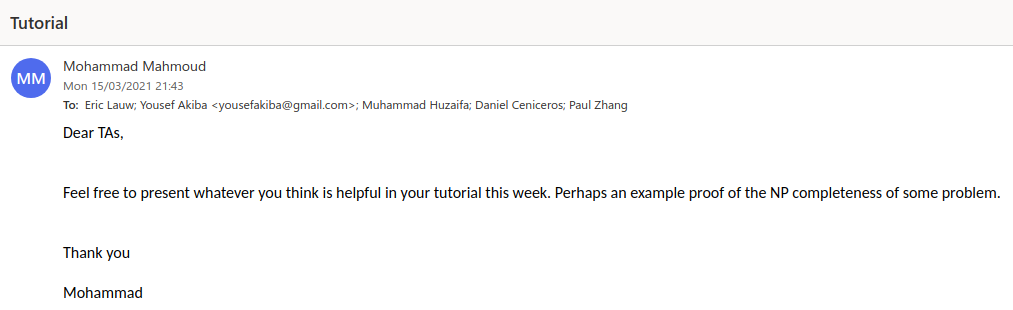
\includegraphics[width=10cm]{img/helpme.png}

D:
\end{figure}

so uh, i hope youse like formulas and logic! phl245 gang \emojisunglasses (even though i havent even taken it before)
\end{frame}

\begin{frame}{formula}
(You'll see the motivation for this section later! it relates to the \textit{3SAT} problem)

\vspace{2mm}

\textbf{Task:} Write out your favourite formula, preferably in \LaTeX, in the chat. My favourite formula is
$$|p_D(n) - r_D(n)| \leq \frac{1}{n^c}.$$
\end{frame}

\begin{frame}{formula}
uh, today we're gonna talk about a different type of formula, probably ;-; we're talking about boolean formulas!\footnote{idk if the plural of formula is ``formulas'' or ``formulae'', not gonna take any sides here.}

\textbf{Definition:} a \textbf{boolean formula} (or \textbf{formula}) is any valid expression involving a bunch of ``boolean variables'' and the operations $\neg, \land, \lor, \Rightarrow, \Leftrightarrow$, and brackets. \footnote{It's kinda an informal definition, but we'll just work with it for now. please accept it.}

\vspace{2mm}

\textbf{Task:} Which of the following are (in your opinion) boolean formulas?
\begin{enumerate}[label=(\alph*)]
\item $x_1 = x_2$.
\item $(x \Rightarrow y) \Leftrightarrow \neg (y \land z)$.
\item $((x \land y) \Rightarrow (x)$.
\item $\Rightarrow \emojisushi \Rightarrow \emojijuice \Rightarrow \emojimoyai$.
\end{enumerate}

\pause

\textbf{Answer:} only $(b)$ is a formula.

\end{frame}

\begin{frame}{formula}
Do you remember truth tables?
\begin{figure}[h]
\centering
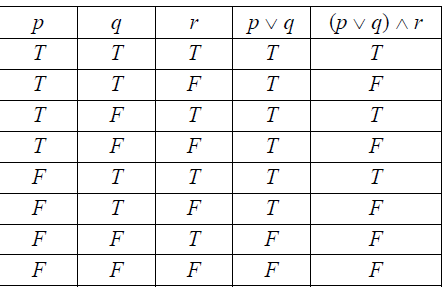
\includegraphics[width=7cm]{img/truth_table.png}
\end{figure}

Let us write out the truth table for $(x \Rightarrow y) \Leftrightarrow \neg (y \land z)$!


\end{frame}

\begin{frame}{formula}
\textbf{Task:} Fill in the following truth table for $(x \Rightarrow y) \Leftrightarrow \neg (y \land z)$.

\begin{center}
\begin{tabular}{|c|c|c|c|}
\hline
$x$ & $y$ & $z$ & $(x \Rightarrow y) \Leftrightarrow \neg (y \land z)$\\
\hline
T & T & T & \\
\hline
T & T & F & \\
\hline
T & F & T & \\
\hline
T & F & F & \\
\hline
F & T & T & \\
\hline
F & T & F & \\
\hline
F & F & T & \\
\hline
F & F & F & \\
\hline
\end{tabular}
\end{center}

\end{frame}

\begin{frame}{formula}
\begin{center}
\begin{tabular}{|c|c|c|c|}
\hline
$x$ & $y$ & $z$ & $(x \Rightarrow y) \Leftrightarrow \neg (y \land z)$\\
\hline
T & T & T & F\\
\hline
T & T & F & T\\
\hline
T & F & T & F\\
\hline
T & F & F & F\\
\hline
F & T & T & F\\
\hline
F & T & F & T\\
\hline
F & F & T & T\\
\hline
F & F & F & T\\
\hline
\end{tabular}
\end{center}
Today's tutorial is sponsored by \texttt{larry.png}. get 60\% off your term test grade with code \texttt{MAXTERM} today. Click the link in the description below.

\begin{figure}[h]
\centering

\includegraphics[width=5cm]{img/larry.png}
\end{figure}

\end{frame}

\begin{frame}{formula}
\begin{center}
\begin{tabular}{|c|c|c|c|}
\hline
$x$ & $y$ & $z$ & $(x \Rightarrow y) \Leftrightarrow \neg (y \land z)$\\
\hline
T & T & T & F\\
\hline
T & T & F & T\\
\hline
T & F & T & F\\
\hline
T & F & F & F\\
\hline
F & T & T & F\\
\hline
F & T & F & T\\
\hline
F & F & T & T\\
\hline
F & F & F & T\\
\hline
\end{tabular}
\end{center}
Anyway, this truth table allows us to turn $(x \Rightarrow y) \Leftrightarrow \neg (y \land z)$ into an equivalent statement written in what's called a \textbf{conjunctive normal form (CNF)}. So $(x \Rightarrow y) \Leftrightarrow \neg (y \land z)$ is \textit{logically equivalent} to the following, which is in CNF:
$$(\neg x \lor \neg y \lor \neg z) \land (\neg x \lor y \lor z) \land (\neg x \lor y \lor z) \land (x \lor \neg x \lor \neg z).$$
\end{frame}

\begin{frame}{formula}
More formally, a \textbf{clause} is several variables connected with $\lor$s with, so something like $(x \land \neg y \land \neg z)$ is a clause. A formula is in \textbf{conjunctive normal form (CNF)} if it comprises several clauses connected with $\land$s, as in 
$$(\neg x \lor \neg y \lor \neg z) \land (\neg x \lor y \lor z) \land (\neg x \lor y \lor z) \land (x \lor \neg x \lor \neg z).$$
\end{frame}

\begin{frame}{formula}
\begin{center}
\begin{tabular}{|c|c|c|c|}
\hline
$x$ & $y$ & $z$ & $(x \Rightarrow y) \Leftrightarrow \neg (y \land z)$\\
\hline
\color{red} T & \color{red} T & \color{red} T & \color{red} F\\
\hline
T & T & F & T\\
\hline
\color{red} T & \color{red} F & \color{red} T & \color{red} F\\
\hline
\color{red} T & \color{red} F & \color{red} F & \color{red} F\\
\hline
\color{red} F & \color{red} T & \color{red} T & \color{red} F\\
\hline
F & T & F & T\\
\hline
F & F & T & T\\
\hline
F & F & F & T\\
\hline
\end{tabular}
\end{center}
How to write out the CNF for a formula?
\begin{enumerate}[label=(\arabic*)]
\item Fill out the truth table for the formula.
\item For each row which ends in `F', take the value of the variables coming before it, and negate them and add `$\lor$'. idk how to describe it, but here's an example. For the third row in our table, we create the expression $(\neg x \lor y \lor \neg z)$.
\item Take all the expressions you've made and add $\land$ between them.
\end{enumerate}
\end{frame}

\begin{frame}{formula}
\textbf{Task: } Write out the CNF for the formula $(x \Leftrightarrow (y \Rightarrow z)) \lor \neg y$.
\begin{center}
\begin{tabular}{|c|c|c|c|}
\hline
$x$ & $y$ & $z$ & $(x \Leftrightarrow (y \Rightarrow z)) \lor \neg y$\\
\hline
T & T & T & \\
\hline
T & T & F & \\
\hline
T & F & T & \\
\hline
T & F & F & \\
\hline
F & T & T & \\
\hline
F & T & F & \\
\hline
F & F & T & \\
\hline
F & F & F & \\
\hline
\end{tabular}
\end{center}
\end{frame}


\begin{frame}{formula}
\textbf{Task: } Write out the CNF for the formula $(x \Leftrightarrow (y \Rightarrow z)) \lor \neg y$.
\begin{center}
\begin{tabular}{|c|c|c|c|}
\hline
$x$ & $y$ & $z$ & $(x \Leftrightarrow (y \Rightarrow z)) \lor \neg y$\\
\hline
T & T & T & T\\
\hline
T & T & F & F\\
\hline
T & F & T & T\\
\hline
T & F & F & T\\
\hline
F & T & T & F\\
\hline
F & T & F & T\\
\hline
F & F & T & T\\
\hline
F & F & F & T\\
\hline
\end{tabular}
\end{center}
So the CNF should be $(\neg x \lor \neg y \lor z) \land (x \lor \neg y \lor \neg z)$.
\end{frame}

\begin{frame}{are you satisfied \emojiflushed}

Now we introduce the \textbf{3SAT problem}. Say you are given a formula in CNF, but in each bracketed term there must be exactly 3 variables. So
\begin{itemize}
\item $(x \Leftrightarrow (y \Rightarrow z)) \lor \neg y$ doesn't work, cuz it's not in CNF.
\item $(x \land y \land \neg z) \lor (\neg x \land \neg y \land \neg z)$ doesn't work, cuz it's not in CNF.
\item $(x \lor y \lor z) \land (y \lor z)$ doesn't work, cuz it doesn't have exactly 3 variables in each bracket.
\item $(x \lor \neg y \lor x) \land (\neg x \lor z \lor \neg w)$ works! (you could have more than 3 variables in the whole expression, and you may repeat variables).
\end{itemize}

So you're given this CNF formula,\footnote{it's in fact called a 3CNF formula!} and you're asked the following question: can you assign truth values to all the variables so that the CNF formula is true? 

\vspace{2mm}

in the example $(x \lor \neg y \lor \neg z) \land (\neg x \lor z \lor \neg w)$, the answer is yes, since if we assign $x, z$ to be true and $y, w$ to be false, then
$(x \lor \neg y \lor \neg z) \land (x \lor z \lor \neg w)$ is true.
\end{frame}

\begin{frame}{are you satisfied \emojiflushed}

So you're given this CNF formula,\footnote{it's in fact called a 3CNF formula!} and you're asked the following question: can you assign truth values to all the variables so that the CNF formula is true? 

\vspace{2mm}

in the example \begin{align*}
&(x \lor y \lor z) \land (x \lor y \lor \neg z) \land (x \lor \neg y \lor z) \land  (x \lor \neg y \lor \neg z)\\
\land &(\neg x \lor y \lor z) \land (\neg x \lor y \lor \neg z) \land (\neg x \lor \neg y \lor z) \land (\neg x \lor \neg y \lor \neg z)
\end{align*}
there is no assignment of variables that makes this true!
\end{frame}

\begin{frame}{are you satisfied \emojiflushed}
turns out, uh, 3SAT\footnote{As a language, 3SAT is defined as $\{\varphi: \text{$\varphi$ is a 3CNF formula that can be satisfied}\}$.} is what is called a \textit{NP-complete problem}. 

\textbf{Definition:} A language $A$ is \textbf{NP-complete} if
\begin{enumerate}[label=(\alph*)]
\item $A \in \text{NP}$;
\item For every $B \in \text{NP}$, $B \leq_p A$.
\end{enumerate}
The above is saying that $A$ is the ``hardest NP problem''. If we can solve $A$ in poly-time, then we can solve \textit{every NP problem in poly-time}, effectively proving P = NP.

\vspace{2mm}

\textbf{Theorem:} 3SAT is NP-complete.

\textbf{Proof:} sorry it's too long and i don't understand it either ;-; it's in the book tho!
\end{frame}

\begin{frame}{np-complete}
3SAT is not the \textit{only} NP-complete problem though! There's a whole plethora of them. They are all \textit{the hardest problems in NP}. If you can solve any one of them in poly-time, then all of them can be solved in poly-time.

\begin{figure}[h]
\centering
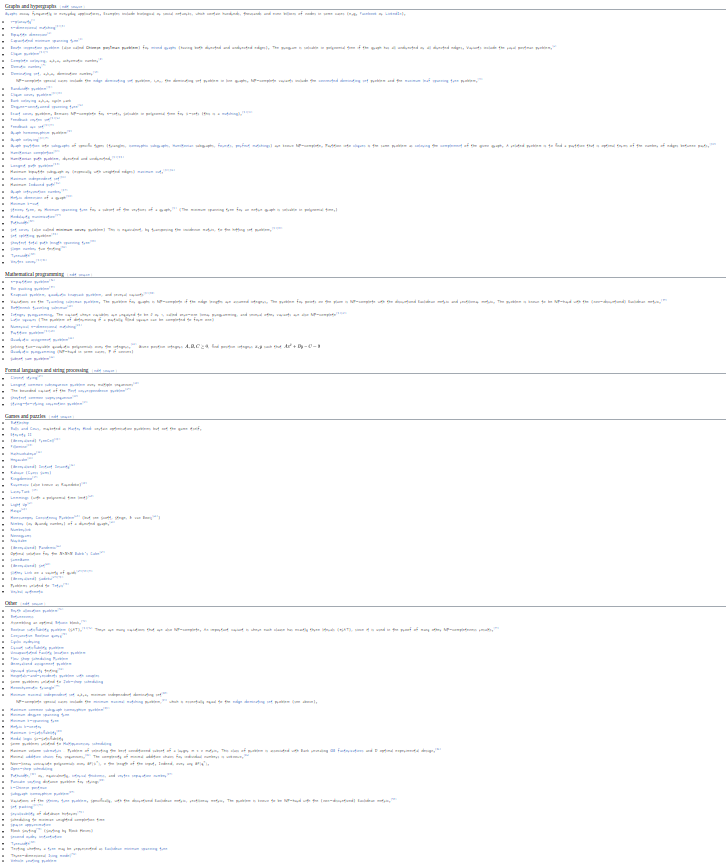
\includegraphics[width=5cm]{img/np-complete.png}
\end{figure}

\end{frame}

\begin{frame}{np-complete}
Basically, if you manage to prove a problem is NP-complete, you shouldn't try to solve it in polynoimal time! If your boss asks you to give a poly-time solution to a NP-complete problem, I'd probably switch employers... cuz that would pretty much amount to proving P = NP, which is really hard! (and if you do manage to prove it, might as well just walk away with the million dollars)

\vspace{2mm}

We'll now prove explain that the \textit{vertex cover problem} is also NP-complete. If you've been in csc373, rejoice! (if you even remember this lol)
\end{frame}

\begin{frame}{cover me owo \emojiflushed}
Let's say you're given an undirected graph $G$. something like
\begin{center}
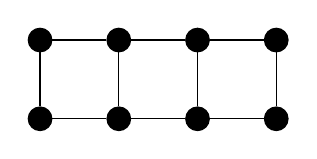
\begin{tikzpicture}[vertex/.style={circle,draw,fill=black,minimum size=3mm,inner sep=3pt]}]
\node[vertex] (v1) at (0, 0) {}; 
\node[vertex] (v2) at (0, 1) {}; 
\node[vertex] (v3) at (1, 0) {}; 
\node[vertex] (v4) at (1, 1) {};
\node[vertex] (v5) at (2, 0) {}; 
\node[vertex] (v6) at (2, 1) {}; 
\node[vertex] (v7) at (3, 0) {}; 
\node[vertex] (v8) at (3, 1) {}; 
\draw 
    (v1) -- (v2) -- (v4)-- (v6) -- (v8) -- (v7) -- (v5) -- (v3) -- (v1)
    (v3) -- (v4)
    (v5) -- (v6);
\end{tikzpicture}
\end{center}

A \textbf{vertex-cover} for $G$ is a set of vertices $V$ in $G$ such that every edge in $G$ touches at least one vertex in $V$. In the graph on the left below, the red vertices form a vertex cover; in the graph on the right, the red vertices don't form a vertex cover.
\begin{center}
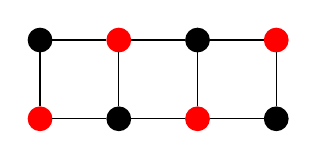
\begin{tikzpicture}[vertex/.style={circle,draw,fill=black,minimum size=3mm,inner sep=3pt]}]
\node[vertex,red] (v1) at (0, 0) {}; 
\node[vertex] (v2) at (0, 1) {}; 
\node[vertex] (v3) at (1, 0) {}; 
\node[vertex,red] (v4) at (1, 1) {};
\node[vertex,red] (v5) at (2, 0) {}; 
\node[vertex] (v6) at (2, 1) {}; 
\node[vertex] (v7) at (3, 0) {}; 
\node[vertex,red] (v8) at (3, 1) {}; 
\draw 
    (v1) -- (v2) -- (v4)-- (v6) -- (v8) -- (v7) -- (v5) -- (v3) -- (v1)
    (v3) -- (v4)
    (v5) -- (v6);
\end{tikzpicture}
\hspace{3mm}
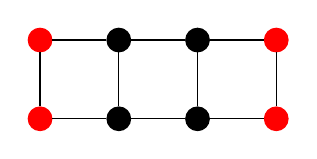
\begin{tikzpicture}[vertex/.style={circle,draw,fill=black,minimum size=3mm,inner sep=3pt]}]
\node[vertex,red] (v1) at (0, 0) {}; 
\node[vertex,red] (v2) at (0, 1) {}; 
\node[vertex] (v3) at (1, 0) {}; 
\node[vertex] (v4) at (1, 1) {};
\node[vertex] (v5) at (2, 0) {}; 
\node[vertex] (v6) at (2, 1) {}; 
\node[vertex,red] (v7) at (3, 0) {}; 
\node[vertex,red] (v8) at (3, 1) {}; 
\draw 
    (v1) -- (v2) -- (v4)-- (v6) -- (v8) -- (v7) -- (v5) -- (v3) -- (v1)
    (v3) -- (v4)
    (v5) -- (v6);
\end{tikzpicture}
\end{center}
The \textbf{size} of a vertex cover is the number of vertices in our vertex cover. The size of the vertex cover on the left graph is 4. (In fact this is the minimum vertex cover size for our graph!)
\end{frame}

\begin{frame}{cover me owo \emojiflushed}
\textbf{Task:} Find a vertex cover for the following graph $G$ (it has four disconnected components). What is the size of the covering? Can you make it smaller?
\begin{center}
\only<1>{
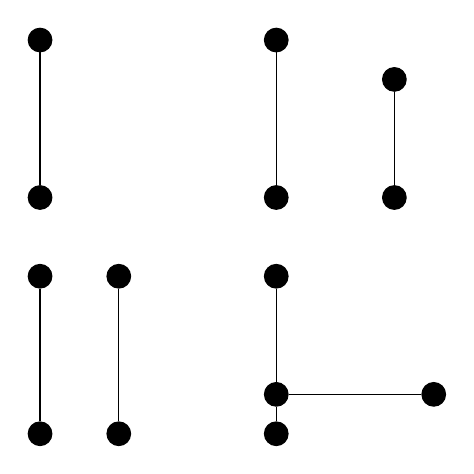
\begin{tikzpicture}[vertex/.style={circle,draw,fill=black,minimum size=3mm,inner sep=3pt]}]
\node[vertex] (v1) at (0, 0) {}; 
\node[vertex] (v2) at (0, 2) {}; 
\node[vertex] (v3) at (1, 0) {}; 
\node[vertex] (v4) at (1, 2) {};
\draw 
    (v1) -- (v2)
    (v3) -- (v4);
\node[vertex] (v5) at (0, 3) {}; 
\node[vertex] (v6) at (0, 5) {}; 
\draw 
    (v5) -- (v6);
\node[vertex] (v7) at (3, 0) {}; 
\node[vertex] (v8) at (3, 2) {}; 
\node[vertex] (v9) at (3, 0.5) {}; 
\node[vertex] (v10) at (5, 0.5) {}; 
\draw 
    (v7) -- (v9) -- (v8)
    (v9) -- (v10);
\node[vertex] (v11) at (3, 3) {}; 
\node[vertex] (v12) at (3, 5) {}; 
\node[vertex] (v13) at (4.5, 3) {}; 
\node[vertex] (v14) at (4.5, 4.5) {}; 
\draw 
    (v11) -- (v12)
    (v13) -- (v14);
\end{tikzpicture}}
\only<2->{
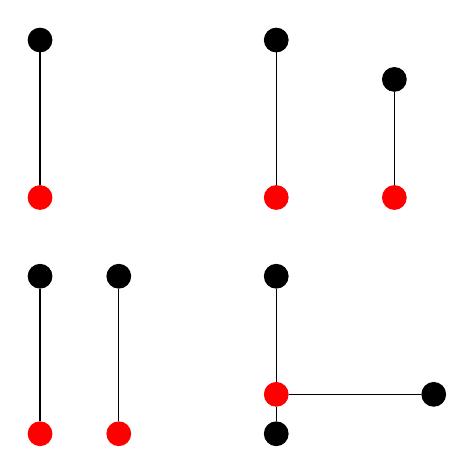
\begin{tikzpicture}[vertex/.style={circle,draw,fill=black,minimum size=3mm,inner sep=3pt]}]
\node[vertex,red] (v1) at (0, 0) {}; 
\node[vertex] (v2) at (0, 2) {}; 
\node[vertex,red] (v3) at (1, 0) {}; 
\node[vertex] (v4) at (1, 2) {};
\draw 
    (v1) -- (v2)
    (v3) -- (v4);
\node[vertex,red] (v5) at (0, 3) {}; 
\node[vertex] (v6) at (0, 5) {}; 
\draw 
    (v5) -- (v6);
\node[vertex] (v7) at (3, 0) {}; 
\node[vertex] (v8) at (3, 2) {}; 
\node[vertex,red] (v9) at (3, 0.5) {}; 
\node[vertex] (v10) at (5, 0.5) {}; 
\draw 
    (v7) -- (v9) -- (v8)
    (v9) -- (v10);
\node[vertex,red] (v11) at (3, 3) {}; 
\node[vertex] (v12) at (3, 5) {}; 
\node[vertex,red] (v13) at (4.5, 3) {}; 
\node[vertex] (v14) at (4.5, 4.5) {}; 
\draw 
    (v11) -- (v12)
    (v13) -- (v14);
\end{tikzpicture}

(size 6)
}
\end{center}

\end{frame}

\begin{frame}{cover me owo \emojiflushed}
The \textbf{vertex cover problem} gives you an arbitrary undirected graph $G$ and an integer $k$, and asks you if there is a vertex cover of size $k$. We can think of this as the language
$$\text{VC} = \{(G, k): \text{$G$ is a graph with a vertex cover of size $k$}\}.$$

Turns out this language is NP-complete! We'll prove it, which involves showing two things:
\begin{itemize}
\item $\text{VC}\in \text{NP}$;
\item $A \leq_p \text{VC}$ for all languages $A \in \text{NP}$.
\end{itemize}

The first one is quick to prove: you can build a poly-time verifier $V$:\footnote{
Recall (from last tutorial) that a language is in NP iff it has a poly-time verifier. A verifier for a language $A$ is a TM $V$ such that
$$A = \{s: \text{there is a string $c$ such that $V(s, c)$ accepts}\}.$$}
\begin{align*}
V(G, k, S): \quad &\text{Check if $S$ is a vertex cover of $V$}\\
&\text{Check if $S$ has size $k$}\\
&\text{Accept iff both conditions are satisfied.}\\
\end{align*}
\end{frame}

\begin{frame}{cover me owo \emojiflushed}
The \textbf{vertex cover problem} gives you an arbitrary undirected graph $G$ and an integer $k$, and asks you if there is a vertex cover of size $k$. We can think of this as the language
$$\text{VC} = \{(G, k): \text{$G$ is a graph with a vertex cover of size $k$}\}.$$

Turns out this language is NP-complete! We'll prove it, which involves showing two things:
\begin{itemize}
\item $\text{VC}\in \text{NP}$;
\item $A \leq_p \text{VC}$ for all languages $A \in \text{NP}$.
\end{itemize}

The first one is quick to prove: you can build a poly-time verifier $V$:\footnote{
Recall (from last tutorial) that a language is in NP iff it has a poly-time verifier. A verifier for a language $A$ is a TM $V$ such that
$$A = \{s: \text{there is a string $c$ such that $V(s, c)$ accepts}\}.$$}
\begin{align*}
V(G, k, S): \quad &\text{Check if $S$ is a vertex cover of $V$}\\
&\text{Check if $S$ has size $k$}\\
&\text{Accept iff both conditions are satisfied.}\\
\end{align*}
\end{frame}

\begin{frame}{cover me owo \emojiflushed}
We now prove $A \leq_p \text{VC}$ for any language $A \in \text{NP}$. In fact, it is sufficient to show $\text{3SAT} \leq_p \text{VC}$: since we know 3SAT is NP-complete, every $A \in \text{NP}$ satisfies $A \leq_p \text{3SAT}$; if $\text{3SAT} \leq_p \text{VC}$ then by transitivity $A \leq_p \text{VC}$ as well!

\vspace{2mm}

From now on this is how we will prove that something is NP-complete: just show some already known NP-complete problem reduces to it.

\vspace{2mm}

To show 3SAT $\leq_P$ VC, we show that if we can solve VC in poly-time, then we can solve 3SAT in poly-time as well.
\end{frame}

\begin{frame}{3SAT $\leq_P$ VC \emojiflushed}
Suppose we can solve VC in poly-time. Given a 3CNF formula $\varphi$, we will construct a graph $G$ as follows:

\begin{figure}[h]
\centering
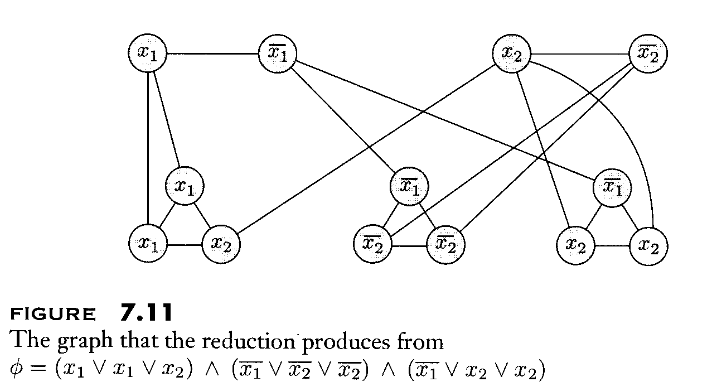
\includegraphics[width=8cm]{img/book_example.png}


(uh, i'm probably just gonna narrate the rest of this! if you're just reading those slides, it's in Sipser's book on pg261)
\end{figure}


\end{frame}

\begin{frame}{\emojimoyai}

bye! D: and hope today's tutorial\footnote{probably more like a lecture disguised as a review session.} wasn't too flushed out.

\begin{figure}[h]
\centering

\includegraphics[width=8cm]{img/not_floppa.png}
\end{figure}

\end{frame}




\end{document}